% $Id:$
%
\documentclass[a4paper,10pt,twoside]{report}
%
\usepackage[english,dutch,ngerman,english]{babel}
\usepackage{microtype}
\usepackage{relsize} %for \textscale{.75}
\usepackage{booktabs}
\usepackage{varioref}
\usepackage[verbose]{geometry}
%
%\usepackage{tikz}
%\usetikzlibrary{shapes.geometric,shapes.arrows,decorations.pathmorphing}
%\usetikzlibrary{matrix,chains,scopes,positioning,arrows,fit}
%
% These three are together:
\usepackage[latin1]{inputenc}
\usepackage[T1]{fontenc}
\usepackage[style=british]{csquotes}
%
\usepackage{color}
\usepackage{url}
\usepackage{sepnum}
\usepackage{appendix}
\usepackage{amssymb} %for twoheadrightarrow 
%
\usepackage{setspace}
\onehalfspacing
%
\usepackage{verbatim}
%
%http://tex.stackexchange.com/questions/18969/creating-a-zebra-effect-using-listings
\usepackage{lstlinebgrd}
%
% ---- Commands/definitions/&c.
%
%\makeatletter
% ----
\newcommand{\cmp}[1]{\texttt{#1}} %%computer (was cmd)
\newcommand{\step}[1]{step \textsf{#1}} %%step 1a->\step{1a}
\newcommand{\topn}[1]{top--\ensuremath{#1}}
\newcommand{\num}[1]{\sepnum{.}{\,}{}{#1}}
\newcommand{\faint}[1]{\color[gray]{0.4}{#1}}
\newcommand{\q}[1]{\enquote{#1}}
\newcommand{\qq}[1]{\enquote*{#1}}
\newcommand{\lf}[0]{\ \\ \noindent}
\newcommand{\lflf}[0]{\ \\ \ \\ \noindent}
\newcommand{\fv}[1]{\emph{#1}} %%feature value
\newcommand{\tv}[1]{\emph{#1}} %%target value
\newcommand{\numexpl}[2]{\ensuremath{#1_{\textrm{\footnotesize{#2}}}}}
%\newcommand{\dist}[2]{\ensuremath{\left(\shortstack[l]{{\sf #1} \\ \small{#2}}\right)}}
\newcommand{\dist}[2]{\scalebox{1.3}{\ensuremath{\frac{\sf #1}{#2}}}}
\newcommand{\inst}[1]{\boxed{\small{{\sf #1}}}} %instance
\newcommand{\targ}[1]{\boxed{\small{{\sf #1}}}} %target
\newcommand{\patt}[2]{\inst{#1}~\targ{#2}} %full pattern
%%                           after Big] \rule[-1mm]{0mm}{4mm}
\newcommand{\dsum}[2]{\ensuremath{\Big]_{#2}^{#1}}} %dist size/fsum
%\newcommand{\pattt}[3]{\inst{#1}~$\frac{{\sf #2}}{{\bf #3}}$} %full pattern
% ----
\newenvironment{varlist}[1]{%
\begin{list}{}{%
    \settowidth{\labelwidth}{\textsf{#1} }     %longest label length
%    \addtolength{\labelsep}{3ex}          %extra space between lbl/txt
    \setlength{\leftmargin}{\labelwidth}  %determine leftmargin
    \addtolength{\leftmargin}{\labelsep}  %determine leftmargin
    \setlength{\parsep}{0.5ex plus 0.2ex minus 0.2ex}
    \setlength{\itemsep}{0.3ex}
    \renewcommand{\makelabel}[1]{\textsf{##1}\hfill}}}%
{\end{list}}
%
\newcounter{exampleno}
\newcommand\theexample{\arabic{exampleno}}
\newenvironment{example}%
{\refstepcounter{exampleno}\vspace{\parsep}\noindent\begin{slshape}}%b
{\hspace{\stretch{1}\end{slshape}(\theexample\vspace{\parsep}}\hspace{\parsep}}%e
%
%
\newenvironment{technical}%
{\begin{slshape}}
{\end{slshape}}
%
\renewcommand\arraystretch{1.1}%
%
\newlength{\pdfwidth}
%%\setlength{\pdfwidth}{1.0\textwidth}
\setlength{\pdfwidth}{0.45\textwidth}
\newlength{\halfpage}
\setlength{\halfpage}{0.5\textwidth}
\newlength{\halfpagefig}
\setlength{\halfpagefig}{0.5\textwidth}
\addtolength{\halfpagefig}{-0.25cm}
\newlength{\thirdpage}
\setlength{\thirdpage}{0.33\textwidth}
%
% from http://blog.pcode.nl/2007/07/19/latex-tips-tricks/:
\renewcommand{\bfdefault}{sb}
%
\newcommand{\boxed}[1]{\fbox{#1\strut}}
% ----
\definecolor{Burgundy}{rgb}{.647,.129,.149}
\definecolor{Grey}{rgb}{.5,.5,.5}
%
\lstnewenvironment{bash}[1]%
{\lstset{aboveskip=\bigskipamount,belowskip=\bigskipamount,numbers=left,numberstyle=\tiny,language=bash,caption=#1,abovecaptionskip=\bigskipamount,basicstyle=\ttfamily\small,linebackgroundcolor={\ifodd\value{lstnumber}\color{green!25}\else\color{green!2}\fi}}}
{}
%
\lstnewenvironment{wout}[1]%
{\lstset{aboveskip=\bigskipamount,belowskip=\bigskipamount,language=bash,caption=#1,basicstyle=\ttfamily\small,linebackgroundcolor={\ifodd\value{lstnumber}\color{black!10}\else\color{black!2}\fi}}}
{}
%
\newcommand{\suchthat}{%
\mathrel{\ooalign{$\omega$\cr\kern-1pt$-$\kern-6.5pt$lp$}}}
\usepackage{accents}
\newcommand{\wlp}{\ensuremath{\accentset{p}{\omega}}}
%\newcommand{\wlp}{\underaccent{px}{\omega}}
%
%--
%    a
\def\ai{\textsc{a.i.}}
\def\asr{\textsc{asr}}
%    b
\def\bleu{\textsc{bleu}}
%    c
\def\cpp{\textsc{c\small{++}}}
\def\cg{correct} %classification
\def\cd{in-distribution}
%    d
\def\DTI{\textsc{dutch-twente-ilk}}
\def\dti{\textsc{dutch-twente-ilk}}
\def\Dimpl{\textsc{Dimpl}}
%    e
\def\ep{\textsc{EuroParl}}
\def\eos{$<$/s$>$}
%\def\etc{\&c}
\def\etc{et cetera}
%    g
\def\gc{global context}
\def\giza{\textsc{giza\small{++}}}
\def\gr{gain ratio}
%    h
\def\hmm{\textsc{hmm}}
%    i
\def\IBo{\textsc{IB1}}
\def\ibo{\textsc{ib\small{1}}}
\def\IBt{\textsc{IB2}}
\def\ibt{\textsc{ib\small{2}}}
\def\ic{incorrect} %classification
\def\IGTree{\textsc{IGTree}}
\def\Igtree{\textsc{Igtree}}
\def\igtree{\textsc{igtree}}
\def\ilk{\textsc{ilk}}
%    k
\def\knn{$k$-\textsc{nn}}
%    l
\def\LM{\textsc{lm}}
\def\lm{language model}
\def\lms{language models}
%    m
\def\mb{memory based}
\def\Mb{Memory based}
\def\mblm{\textsc{mblm}}
\def\mbmt{\textsc{mbmt}}
\def\meteor{\textsc{meteor}}
\def\mono{monolithic}
\def\Moses{\textsc{Moses}}
\def\moses{\textsc{moses}}
\def\mrr{\textsc{mrr}}
\def\mt{\textsc{mt}}
%    n
\def\nist{\textsc{nist}}
\def\ngram{$n$-gram}
\def\Ngram{$N$-gram}
\def\nlp{natural language processing}
%    p
\def\per{\textsc{per}}
\def\pid{\textsc{pid}}
\def\pbmbmt{\textsc{pbmbmt}}
%    r
\def\rr{reciprocal rank}
%    s
\def\Smt{\textsc{Smt}}
\def\smt{\textsc{smt}}
\def\Srilm{\textsc{Srilm}}
\def\srilm{\textsc{srilm}}
\def\sos{$<$s$>$}
%    t
\def\Timbl{\textsc{Timbl}}
\def\timbl{\textsc{timbl}}
\def\tribl{\textsc{tribl}}
\def\Triblt{\textsc{Tribl\small{2}}}
\def\triblt{\textsc{tribl\small{2}}}
%    u
\def\unix{\textsc{unix}}
%    w
\def\wer{\textsc{wer}}
\def\Wopr{\textsc{Wopr}}
\def\wopr{\textsc{wopr}}
\def\wex{word expert}
\def\Wex{Word expert}
\def\wexs{word experts}
%--

% -*- tex -*-
%
\usepackage{ifthen}

\usepackage{tikz}
\usetikzlibrary{shapes,shadows,chains,shapes.multipart,arrows,positioning,fit}


\tikzstyle{inf} = [chamfered rectangle corners=north west, draw,text depth=.25ex]

\tikzstyle{lhs} = [signal, signal pointer angle=145,draw,signal to=nowhere,node
distance=0mm,text height=1.5ex,text depth=.25ex, signal from=east]

\tikzstyle{tgt} = [signal, signal pointer angle=145 , draw, signal to=nowhere,node distance=0mm,text height=1.5ex,text depth=.25ex, signal to=west,signal to=east,fill=gray!20]

\tikzstyle{rhs} = [signal, signal pointer angle=145 , draw, signal to=nowhere,node distance=0mm,text height=1.5ex,text depth=.25ex, signal from=west]

\tikzstyle{cls} = [rectangle, draw,node distance=0mm,text height=1.5ex,text depth=.25ex]
%different styles for cg, cd etc.^^

\tikzstyle{dist} = [rectangle,node distance=1mm,minimum size=6mm]

\begin{comment}
\begin{tikzpicture}
\node[lhs] (n0) {left hand side};
\node[tgt] (n1) [right=of n0] {target};
\node[rhs] (n2) [right=of n1] {foo};
\node[cls] (n3) [right=of n2] {bar};
\node[dist] (txt) [right=of n3] {\dist{the}{10}\dist{a}{9}\dist{in}{8}\dsum{1}{1}};
\end{tikzpicture}
\end{comment}



%wopr out: { W/M }{ CG/CD/IC }{ LHS }{ TARGET }{ RHS }{ CLASS }{ DISTR }
%            1       2          3      4         5       6       7
\newcommand{\wlr}[7]{\noindent\ensuremath{\begin{tikzpicture}
% first a place holder, haf the size of the WEX circle, so the
% WEX and  MONO boxes align.
\ifthenelse{\equal{#1}{w}}{
  \node (sp) [draw,fill=white,circle,inner sep=0pt,minimum size=0pt] {};
}{
  \node (sp) [draw=white,fill=white,circle,inner sep=0pt,minimum size=1.5pt] {};
}
% end if
\node[lhs] (n0) [right=of sp] {{\sf #3}};
% print dot if WEX (open dot if MONO, then we don't need (sp) ?)
\ifthenelse{\equal{#1}{w}}{
  \node (c1) at (n0.north west) [draw,fill,circle,inner sep=0pt,minimum size=3pt] {};
}{}
% end if
\node[tgt] (n1) [right=of n0] {{\sf #4}};
% RHS? If empty {}, skip, print rest
\ifthenelse{\equal{#5}{}}{
  \node[cls] (n3) [right=of n1] {{\sf #6}};
}{ % We do have a RHS
  \node[rhs] (n2) [right=of n1] {{\sf #5}};
  \node[cls] (n3) [right=of n2] {{\sf #6}};
} % end if RHS
% cross out if wrong answer
\ifthenelse{\equal{#2}{ic}}{
  \draw (n3.north east) -- (n3.south west);
}{}
% end if
% dotted if cd
\ifthenelse{\equal{#2}{cd}}{
  \draw [dotted, thick] (n3.north east) -- (n3.south west);
}{}
% end if
\node[dist] (txt) [right=of n3] {#7};
\end{tikzpicture}}}


% Instance
%
\newcommand{\tri}[3]{\makebox[1.5cm][l]{#1}\makebox[1.5cm][l]{#2}\makebox[1.5cm][l]{#3}}
\newcommand{\trit}[1]{\makebox[1.5cm][l]{#1}}
%
%instance l3
\newcommand{\ilt}[4]{\noindent\ensuremath{\begin{tikzpicture}
\node [rectangle, node distance=0mm,text height=1.5ex,text
depth=.25ex, draw] (i) {\tri{#1}{#2}{#3}};
\node [rectangle, node distance=0mm,text height=1.5ex,text depth=.25ex
, draw] (n1) [right=of i] {\trit{#4}};
\end{tikzpicture}}}
%
\newcommand{\bit}[1]{
\node [rectangle, node distance=0mm,text height=1.5ex,text depth=.25ex
, draw] {\bbx{#1}};
}
\newcommand{\OLDtrigram}[4]{\noindent\ensuremath{\begin{tikzpicture}
\bit{#1}\bit{#2}\bit{#3}\bit{#4}
\end{tikzpicture}}}
%
%%%
%
\newcommand{\bbx}[1]{\makebox[1.25cm][l]{\footnotesize{\sf #1}}}
\newcommand{\trigram}[4]{\noindent
\begin{tikzpicture}[start chain,node distance=1mm]
\node [on chain, drop shadow, rectangle, node distance=0mm,text height=1.5ex,text depth=.25ex
, draw, fill=white] {\bbx{#1}};
\node [on chain, drop shadow, rectangle, node distance=0mm,text height=1.5ex,text depth=.25ex
, draw, fill=white] {\bbx{#2}};
\node [on chain, drop shadow, rectangle, node distance=0mm,text height=1.5ex,text depth=.25ex
, draw, fill=white] {\bbx{#3}};
\node [on chain, drop shadow, rectangle, node distance=0mm,text height=1.5ex,text depth=.25ex
, draw, fill=gray!20] {\bbx{#4}};
\end{tikzpicture}
}


%\makeatother
%
% Chapter/section style
\usepackage{pbstyle}
% ----

%%I'm afraid that if you look at a thing long enough, it loses
%% all of its meaning. --Andy Warhol

\begin{document}

\title{Wopr}
\author{Peter Berck}
\date{\today}

\maketitle

%% ----------------------------------------------------------------
%\makeemptypage
\clearpage
\tableofcontents

%% ---

\chapter{Intro}

\Wopr{} is a wrapper around the \knn{} classifier in \Timbl{},
offering word prediction and language modeling
functionalities. Trained on a text corpus, \wopr{} can predict missing
words, report perplexities at the word level and the text level, and
generate spelling correction hypotheses.

\par
Besides the \Timbl{}-related functionality, \wopr{} can create and
manipulated data sets.

\par

\Mb{} word prediction illustrates an interesting idea. Complex
abstraction levels are not needed for (some) linguistic
tasks. In the case of word prediction, the words themselves provide
enough information. To put it bluntly, we generalise without
abstracting. 

\par
This manual is divided into several parts. Chapter Two contains a walk
through illustrating the main use cases of \wopr{}. Chapter Three
shows how to compile and install \wopr{}. Chapter Four has some
information about the performance of \wopr{}, and compares the output
to \srilm{} output. Finally, Chapter Five contains a more detailed
reference or some of the \wopr{} functions.

\par
This manual assumes familiarity with language modeling in
general. Experience with memory based based learning techniques (or
with \Timbl{}) is an distinct advantage.

% word pred: archetypal problem of NLP (Even-Zohar, Roth, Zelenko, 1999
% Many classes, zipfian distr, same as the feature values

\chapter{Walk Throughs}

Without further ado, we present a number of common tasks which can be
performed with \wopr{}. We'll jump right in, and explain the different
steps and option on the way.

\section{Memory Based Language Model}

A memory based version of a trigram model. The following text corpora
are used in the experiments; \cmp{rmt.5e5} for our training data, and
\cmp{rmt.t1000} to test on. The former consists of the first
\num{500000} lines of the Reuters Newspaper corpus, while the latter
contains the last \num{1000} lines.

The following steps are typically taken when creating a model from
scratch.

\begin{varlist}{m}
\item[1] Create a lexicon
\item[2] Create a windowed data set (both for training and testing)
\item[3] Train the instance base
\item[4] Run a prediction test on test data set
\end{varlist}

The lexicon is created as follows.

\begin{bash}{Creating a lexicon}
wopr -r lexicon -p filename:rmt.5e5
\end{bash}

This will create a frequency list of all the tokens in the specified
file. Before we explain what we did, we will show the second step.

%\begin{lstlisting}[language=C,basicstyle=\ttfamily,numberstyle=\zebra{green!25}{green!2},numbers=left]
\begin{bash}{Creating a data set}
wopr -r window_lr -p filename:rmt.5e5,lc:2,rc:0
\end{bash}

These examples shows how \wopr{} is typically used. The two main
points to note are \cmp{-r window\_lr}, and the \cmp{-p \ldots}. The
\cmp{-r} tells \wopr{} to run the \cmp{window\_lr}
function. Everything that follows after \cmp{-p} are the parameters
passed to the function. The parameters are specified as a comma
seperated list of \cmp{keyword:value} pairs. In this case, we specify
a \cmp{filename}, \cmp{rmt.5e5} and the size of the left- and right
contexts. The context consists of two words on the left of the target,
and none on the right. This is abbreviated as \cmp{l2r0}.

\Wopr{} is quite verbose:

\begin{bash}{\Wopr{} output}
wopr -r window_lr -p filename:rmt.5e5,lc:2,rc:0
06:58:37.21: Timbl support built in.
06:58:37.22: /Users/pberck/local/
06:58:37.22: Starting wopr 1.29.3
06:58:37.22: PID:   7433 PPID:   2142
06:58:37.22: Starting.
06:58:37.22: Running: window_lr
06:58:37.22: window_lr
06:58:37.22:  filename:  rmt.5e5
06:58:37.22:  lc:        2
06:58:37.22:  rc:        0
06:58:37.22:  to:        0
06:58:37.22:  OUTPUT:    rmt.5e5.l2r0
06:59:15.61: SET filename to rmt.5e5.l2r0
06:59:15.61: Result = 0
06:59:15.61: Running for 38s
06:59:15.61: Ready.
\end{bash}

Note lines 13 and 14. In line 13, \wopr{} prints the name of the
output file it creates. These filenames are generated automatically by
\wopr{} and contain information about the parameters used. In the case
of \cmp{window\_lr}, it incorporates the context size in the file
name. This allows \wopr{} to skip steps in its processing if they have
been done before. Running the exact same command again will show the
following:

\begin{bash}{}
wopr -l -r window_lr -p filename:rmt.5e5,lc:2,rc:0
07:15:36.38: Running: window_lr
07:15:36.38: window_lr
07:15:36.38:  filename:  rmt.5e5
07:15:36.38:  lc:        2
07:15:36.38:  rc:        0
07:15:36.38:  to:        0
07:15:36.38:  OUTPUT:    rmt.5e5.l2r0
07:15:36.38: OUTPUT exists, not overwriting.
07:15:36.38: SET filename to rmt.5e5.l2r0
07:15:36.38: Result = 0
\end{bash}

Another thing to notice is the \cmp{SET} statement in line
\num{10}. This is useful when combining the different steps. This will
be explained later.

The next step is the creation of the instance base (output has been
reduced to improve readability).

\begin{bash}{Creating an instance base}
wopr -l -r make_ibase -p filename:rmt.5e5.l2r0,timbl:"-a4 +D"
10:02:16.99: Running: make_ibase
10:02:16.99: make_ibase
10:02:16.99:  timbl:     -a4 +D
10:02:16.99:  filename:  rmt.5e5.l2r0
10:02:16.99:  ibasefile: rmt.5e5.l2r0_-a4+D.ibase
...
Size of InstanceBase = 3366271 Nodes, (134650840 bytes), 29.46 % compression
Learning took 527 seconds, 732 milliseconds and 483 microseconds
Writing Instance-Base in: rmt.5e5.l2r0_-a4+D.ibase
10:12:57.87: SET ibasefile to rmt.5e5.l2r0_-a4+D.ibase
10:12:57.87: Result = 0
\end{bash}

Creating the instance based is delegated to \Timbl{}. We refer to
\cite{Daelemans+09} for a thorough explanation. The variables
specified in the \cmp{timbl} parameter are passed verbatim to \Timbl{}.

%The \cmp{\ldots} show where \Timbl{}, which is used by \wopr{} to
%train the instance base, prints its output.

And finally, we use this instance base to run a perplexity calculation
on a test set. The test set has been prepared in a step not shown
here, in the same format as the training data. It contains the last
\num{1000} lines of the Reuters data. Here we also specify the lexicon
created in step \textsf{1}. The lexicon is used to determine if a word
is known or unknown to the system.

\begin{bash}{Running a test}
wopr -l -r pplxs -p ibasefile:rmt.5e5.l2r0_-a4+D.ibase,
                    filename:rmt.t1000.l2r0,timbl:"-a4 +D",
                    lexicon:rmt.5e5.lex
...
11:50:10.93:  Correct:       3368 (20.5893)
11:50:10.93:  Correct Distr: 6250 (38.2076)
11:50:10.93:  Correct Total: 9618 (58.7969)
11:50:10.93:  Wrong:         6740 (41.2031)
11:50:10.93:  Timbl took: 11m47s
11:50:10.93:  SET px_file to rmt.t1000.l2r0_11615.px
11:50:10.93:  SET pxs_file to rmt.t1000.l2r0_11615.pxs
11:50:11.09: Result = 0
\end{bash}

\Wopr{} generates two output files. The important one is
\cmp{rmt.t1000.l2r0\_11615.px}. That contains the prediction and
statistics for each test instance we processed.

An extra perl script, \cmp{pplxs\_px.pl} has been supplied to post
process the output. It can be found in the \cmp{etc/} directory in the
\wopr{} distribution. It computes perplexity and other statistics on
the output. It is run as follows.

\begin{bash}{Post processing of \wopr{} output}
perl pplx_px.pl -f rmt.t1000.l2r0_11615.px -l2 -r0
\end{bash}

The file to process is specified with the \cmp{-f} parameter. The
context size is specified with the \cmp{-l} and \cmp{-r}
parameters. It contains a line for each instance, followed by a
summary. A fragment of the output:

\begin{wout}{}
0.02119694  -5.5600  -1.6737  1 1 [01010] ways
0.41176411  -1.2801  -0.3854  1 1 [01010] of
\end{wout}

It shows the probability of the classification, followed by the
$log_2$ and $log_{10}$ of the probability. For an explanation of the
other values, see the reference chapter. The summary at the end shows,
amongst other statistics, the perplexity on the test data.

\begin{wout}{}
Wordcount: 16358 sentencecount: 0 oovcount: 542
Wopr ppl:    251.41 Wopr ppl1:    251.41  (No oov words.)
\end{wout}

To get performance per word, the \cmp{-w} flag can be added.

\begin{wout}{}
winner: cg:0 (0.00%) cd:0 (0.00%) ic:1 (100.00%)
with: cg:11 (18.33%) cd:22 (36.67%) ic:27 (45.00%)
\end{wout}

This show that the word \cmp{winner} appeared once in the test set,
and was incorrectly predicted. The word \cmp{with} was predicted
correctly in \num{11} cases, \etc{}.

\subsection{Multiple Test Files}

Instead of processing just one file, a directory argument can be given
to \wopr{} to process all files matching a certain expression.

\begin{bash}{Processing multiple files}
wopr -l -r pplxs -p ibasefile:rmt.5e5.l2r0_-a4+D.ibase,
                    dir:expdir,timbl:"-a4 +D",
                    lexicon:rmt.5e5.lex
...
13:28:05.56:  dir:             expdir
13:28:05.56:  dirmatch:        .*
13:28:05.56: Processing 1 files.
...
13:28:34.65: Processing: expdir/rmt.t1000.l2r0
13:28:34.65: OUTPUT:     expdir/rmt.t1000.l2r0_4713.px
13:28:34.65: OUTPUT:     expdir/rmt.t1000.l2r0_4713.pxs
...
\end{bash}

Lines five and six show the directory, and the expression used to
match the files. The default is to take all the files in the
directory. To specify something else the parameter \cmp{dirmatch} can
be specified. To process all files ending in \cmp{l2r0}, the
expression \cmp{l2r0\$} can be supplied.

Line seven shows there is only one file, and the rest of the output
shows that each file is processed in a similar manner to the single
file method.

\subsection{Combining Commands}

As we mentioned before, the \wopr{}-commands can be combined. \Wopr{}
has a mechanism to automatically generate output filenames based on
certain parameters. It will \q{create} come of these parameters after
each run, so they will be available to the next function as input
without having to specify them from the start. We can combine several
of the steps we shows in the previous part like this.

\begin{bash}{Combining commands}
wopr -r lexicon,window_lr,make_ibase,pplxs -p filename:rmt.5e5,
                                              timbl:"-a4 +D",lc:2,rc:0
...
09:11:54.15: SET ibasefile to rmt.5e5.l2r0_-a4+D.ibase
09:11:54.15: Result = 0
09:11:54.15: Running: pplxs
09:11:54.15: pplxs
09:11:54.15:  ibasefile:      rmt.5e5.l2r0_-a4+D.ibase
09:11:54.15:  lexicon:        rmt.5e5.lex
09:11:54.15:  counts:         rmt.5e5.cnt
...
\end{bash}

If we look at the last step, \cmp{pplxs}, we see that the instance
base filename and the other parameters have been taken from the
previous steps. This example also shows theproblem with this
mechanism; we cannot generate the windowed test set in the same
chain. That has to be done seperately. (To be clear, one would not run
the example in real life. It was to show both the strength and
weakness of the combined commands.) For complex \wopr{} usage,
\emph{scripting} can (should) be used.

For complex \wopr{} usage, \emph{scripting} can (should) be used.

\section{\ngram{}-model}

\Wopr{} can also create a classical \ngram{}-model. This functionality
has been included so as to be able to compare the \mb{} \lm{} to a 
\q{pure} \ngram{}-model. It has neither been optimised for speed,
nor for memory efficiency.

Creation of the model consists of one step; \cmp{ngl}.

\begin{bash}{Creation of an \ngram{} model}
wopr -r ngl -p filename:rmt.5e5
11:19:40.16: Running: ngl
11:19:40.18: ngl
11:19:40.18:  filename:  rmt.5e5
11:19:40.18:  n:         3
11:19:40.18:  fco:       0
11:19:40.18:  OUTPUT:    rmt.5e5.ngl3f0
11:19:40.18: Reading...
11:21:33.15: Writing...
11:22:36.35: SET ngl to rmt.5e5.ngl3f0
11:22:45.65: Result = 0
\end{bash}

The output contains a list with all the \ngram{}s followed by a
frequency count and a conditional probability. The default \ngram{}
size is three. Instead of the plain probability, the $log_2$ or
$log_{10}$ of the probabilities can be output as well. Use the
\cmp{log} parameter to specify the base of the log.

The command to process a test file is called \cmp{ngt}.

\begin{bash}{testing with an \ngram{} model}
wopr -r ngt -p ngl:rmt.5e5.ngl3f0,testfile:rmt.t1000,topn:3
11:31:50.24: Running: ngt
11:31:50.24: ngt
11:31:50.24:  filename:  rmt.t1000
11:31:50.24:  ngl file:  rmt.5e5.ngl3f0
11:31:50.24:  ngc file:    
11:31:50.24:  n:         3
11:31:50.24:  id:
11:31:50.24:  topn:      3
11:31:50.24:  mode:      wopr
11:31:50.24:  OUTPUT:    rmt.t1000.ngt3
11:31:50.24:  OUTPUT:    rmt.t1000.ngp3
11:31:50.24:  OUTPUT:    rmt.t1000.ngd3
11:31:50.24: Reading ngrams...
11:31:59.71: Writing output...
11:32:00.02: Total words: 16358
11:32:00.02: Total oovs: 542
11:32:00.02: Total log2prob: -121551
11:32:00.02: Average log2prob: -7.6853
11:32:00.02: Average pplx: 205.828
11:32:00.02: SET ngt_file to rmt.t1000.ngt3
11:32:00.02: SET ngp_file to rmt.t1000.ngp3
11:32:00.02: SET ngd_file to rmt.t1000.ngd3
11:32:01.90: Result = 0
\end{bash}

This produces three output files. One, \cmp{rmt.t1000.ngt3}, contains
statistics for each classification, as shown in the following
fragment. It shows a word, the \ngram{} probability, the size of the
matching \ngram{} and the \ngram{} itself.

\begin{wout}{}
and 0.0928793 2 puts and
calls 0.5 3 puts and calls
\end{wout}

The second, \cmp{rmt.t1000.ngp3}, contains statistics per line of text.

\begin{wout}{}
-81.9518 293.087 10 0 The officers quickly managed to calm down ...
\end{wout}

The output contains the entropy, perplexity, word count and number of
unknown words, followed by the text line itself.

The third file, \cmp{rmt.t1000.ngd3}, is a file containing
distributions of possible answers.

\begin{wout}{}
million 0.6 3 9 45 1 [ million 27 mln 6 to 3 ]
eight-year 0.000502681 2 680 5678 0.0208333 [ ) 342 . 342 in 326 ]
bond 0.142857 2 5 7 0.5 [ Eurobond 3 bond 1 contract 1 ]
\end{wout}

It contains the target word, the probability of the classification (or
logprob, if the \cmp{log} parameter has been specified), followed by
the $n$ of the matching \ngram{}, the size of the distribution, the
sum of the frequencies in the distribution, and the reciprocal rank of
the target in the distribution. This is followed by the \topn{n} of
the distribution.

The \cmp{ngt} function can also read and process a language model generated by
\srilm{}. The \srilm{} model needs to have been generated with the
\cmp{-write} option to generate a list with \ngram{} frequency
counts. That file needs to be read with the \cmp{ngc} option. 

%/Users/pberck/work/srilm1.5.7/bin/macosx/
\begin{bash}{Using an \srilm{} language model}
ngram-count -no-eos -no-sos -text TXT -sort -write TXT.ngc -lm TXT.lm
wopr -r ngt -p ngl:TXT.lm,testfile:rmt.t1000,topn:3,mode:srilm,ngc:TXT.ngc
\end{bash}

Using the \cmp{srilm} option sets the system to read and write
the $log_{10}$ of the probabilities. This works also with the \wopr{}
generated \ngram{}s generated with \cmp{ngl}. In both the \cmp{ngl}
and \cmp{ngt} functions the base of the logarithms can be specified
with the \cmp{log} parameter. 

\section{Text Generation}

\Wopr{} can also be used in reverse, and generate text from a
\lm{}. The command is called \cmp{generate}.

\begin{bash}{Text generation}
wopr -r generate -p ibasefile:rmt.5e5.l2r0_-a4+D.ibase,timbl:'-a4 +D',
                    filename:out1,ws:2
\end{bash}

The command still uses the older specification for context,
\cmp{ws}. It needs to be set to the sum of the left and right context
specifiers. 

\begin{wout}{}
Kodjo took the loss , no delays . 
USA : U.S. farm commodities to Russia , China . 
The state had to evacuate the church for two consecutive terms in an 
   abandoned car in the market moved in and out of parliament Koigi 
   wa Wamwere and two hawks on to Baltimore . 
The other 14 first list equities were unchanged in higher management
   ranks . 
\end{wout}


\section{Spelling Correction}

\Wopr{} can also be used to do spelling correction. The correction
algorithm is based on words in the predicted list of words. A filter
is applied to the list, removing words which fall outside predefined
parameters such as levenshtein distance, word length and frequency.

\begin{bash}{Spelling correction}
wopr -r correct -p ibasefile:rmt.5e5.l2r0_-a4+D.ibase,timbl:"-a4 +D",
                   filename:rmt.t1000.l2r0
14:16:50.07: Running: correct
14:16:50.07: correct
14:16:50.07:  ibasefile:  rmt.5e5.l2r0_-a4+D.ibase
14:16:50.07:  lexicon:    
14:16:50.07:  counts:     
14:16:50.07:  timbl:      -a4 +D
14:16:50.07:  id:         7272
14:16:50.07:  mwl:        5
14:16:50.07:  mld:        1
14:16:50.07:  max_ent:    5
14:16:50.07:  max_distr:  10
14:16:50.07:  min_ratio:  0
14:16:50.07: Processing 1 files.
...
14:17:13.02: Processing: rmt.t1000.l2r0
14:17:13.02: OUTPUT:     rmt.t1000.l2r0_7272.sc
...
14:35:42.79:  SET sc_file to rmt.t1000.l2r0_7272.sc
14:35:42.80: Result = 0
\end{bash}

The statistics printed (here removed) can be ignored. The output will
contain a list with the words falling within the parameters. They are
potential corrections of misspelt words.

Reuters doesn't contain misspellings, so we show output from another
file.

\begin{wout}{}
_ _ Her ssiter (sister) -6.26454 0 76.88 1 [ sister 1 ]
\end{wout}

It shows the instance, followed by the classifiers best guess between
parenthesis. This is followed by the logprob, the entropy and the word
logprob ($2^{-logprob}$). The final number is the size of the \Timbl{}
distribution returned, followed by a list with potential misspellings.

\section{Global Context}

\Wopr{} contains a mechanism to include a larger, \emph{global}
context in the classifier. This is done by marking words from a list
with words that are deemed important. When going through a text to
make instances, we put the words from the list we encounter in the
text in the global context. The global context has a certain size, so
that older words are pushed out by newer words. We also put a decay
factor on the words, so that they will disappear even if they are not
pushed out by newer words. These global context instances can be seen
as instances with gaps in them (after all, we don't include every
word), and the idea is that they capture the essence of the
(preceeding) text. The gaps are of variable length, so they have been
dubbed \emph{elastigrams}. To create the instances for \Timbl{}, we
add the global context instances to already existing \q{normal}
instances (in fact, the global context instances are created from a
regular data set).

There is a function to create the global context called
\cmp{lcontext}, and one to create a list with important words from the
lexicon, called \cmp{rfl}.

The steps involved are the following.

\begin{varlist}{m}
\item[1] create training data
\item[2] create a list
\item[3] create the global context from the list and training data
\end{varlist}

The first steps have been explained before, and will just be mentioned
here.

\begin{bash}{Creating lexicon and training data}
wopr -r lexicon -p filename:rmt.5e5
wopr -r window_lr -p filename:rmt.5e5,lc:2,rc:0
\end{bash}

In the next step, we create a list with words which we want to include
in our global context. We take a part of the lexicon, namely from the
50th most frequent word to the 550th most frequent word. We skip the
top-50 words because these are function words, and deemed less
important when trying to catch the essence of the text. The list will
still not be perfect, but serves our purpose.

\begin{bash}{Creating list for global context training data}
wopr -r rfl -p lexicon:rmt.5e5.lex,m:50,n:550
...
10:53:37.62: range_from_lex
10:53:37.62:  lexicon: rmt.5e5.lex
10:53:37.62:  m:       50
10:53:37.62:  n:       550
10:53:37.62:  OUTPUT:  rmt.5e5.lex.r50n550
10:53:37.62: Reading lexicon.
10:53:37.95: Read lexicon.
10:53:38.19: Frequency list: 1786 items.
10:53:38.25: Range file contains 539 items.
10:53:38.25: SET range to rmt.5e5.lex.r50n550
10:53:38.34: Result = 0
\end{bash}

The first five word in the file are:

\begin{wout}{}
year 17964
U.S. 17870
market 17175
but 16501
after 16004
\end{wout}

Now we can combine the list and the training data to form the global
context training data.

\begin{bash}{Creating global context training data}
wopr -r lcontext -p range:rmt.5e5.lex.r50n550,filename:rmt.5e5.l2r0,
                    gcd:50,gcs:10
...
10:58:39.91: lcontext
10:58:39.91: Reading range file.
10:58:39.91: Loaded range file, 539 items.
10:58:39.91:  filename:  rmt.5e5.l2r0
10:58:39.91:  range:     rmt.5e5.lex.r50n550
10:58:39.91:  gcs:       10
10:58:39.91:  gcd:       50
10:58:39.91:  gct:       0
10:58:39.91:  from_data: true
10:58:39.91:  gc_sep:    true
10:58:39.91:  OUTPUT:    rmt.5e5.l2r0.gc10d50t0
11:01:34.19: SET filename to rmt.5e5.l2r0.gc10d50t0
11:01:34.72: Result = 0
\end{bash}

The following shows a fragment of the resulting data set. In line two,
the word \cmp{markets} is (again) added to the head of the global context
part of the instance (fourth word from the right). In line three \cmp{into}
is added, and everything shifts a place to the left.

\begin{wout}{}
_ _ _ _ _ _ markets markets economy back sent Mexican markets
_ _ _ _ _ markets markets economy back markets Mexican markets into
_ _ _ _ markets markets economy back markets into markets into a
_ _ _ _ markets markets economy back markets into into a buzz
\end{wout}

Finally, we create a new instance base, and run a word prediction
experiment.

\begin{bash}{Creating global context training data}
wopr -r make_ibase -p filename:rmt.5e5.l2r0.gc10d50t0,timbl:'-a4 +D'
11:07:57.72: Timbl support built in.
11:07:57.72: /Users/pberck/local/
11:07:57.72: Starting wopr 1.29.3
11:07:57.72: PID:   9161 PPID:   4617
11:07:57.72: Starting.
11:07:57.72: Running: make_ibase
11:07:57.72: make_ibase
11:07:57.72:  timbl:     -a4 +D
11:07:57.72:  filename:  rmt.5e5.l2r0.gc10d50t0
11:07:57.72:  ibasefile: rmt.5e5.l2r0.gc10d50t0_-a4+D.ibase
...
11:20:12.39: SET ibasefile to rmt.5e5.l2r0.gc10d50t0_-a4+D.ibase
11:20:12.39: Result = 0
\end{bash}

\begin{bash}{Creating global context training data}
/exp/pberck/wopr/wopr -l -r pplxs -p filename:rmt.t1000.l2r0.gc10d50t0,
              timbl:"-a4 +D",ibasefile:rmt.5e5.l2r0.gc10d50t0_-a4+D.ibase,
              lexicon:rmt.5e5.lex
...
11:58:55.32: Processing: rmt.t1000.l2r0.gc10d50t0
11:58:55.32: OUTPUT:     rmt.t1000.l2r0.gc10d50t0_30826.px
11:58:55.32: OUTPUT:     rmt.t1000.l2r0.gc10d50t0_30826.pxs
12:51:30.18:  Correct:       3141 (19.2016)
12:51:30.18:  Correct Distr: 866 (5.29405)
12:51:30.18:  Correct Total: 4007 (24.4957)
12:51:30.18:  Wrong:         12351 (75.5043)
12:51:30.18:  Timbl took: 52m25s
12:51:30.18:  SET px_file to rmt.t1000.l2r0.gc10d50t0_30826.px
12:51:30.18:  SET pxs_file to rmt.t1000.l2r0.gc10d50t0_30826.pxs
12:51:30.24: Result = 0
\end{bash}

There are a number of parameters that can be tweaked to get a better
peformance. We refer to the reference section for details.

\section{Multi-classifiers}

\Wopr{} contains functionality to apply more than one classifier on a
task. One modus operandus is to apply multiple classifiers and combine
the different outputs, another is to use a gated approach, and choose
a certain classifier based on context features.

The instance bases and parameters are stored in a configuration file
which is read by \wopr{}.

\subsection{md/md2} %muldi_dist2: md2 and mc

%multi_dists, multi_classifiers?

The following shows a configuration file to apply two different
classifiers to a test set in two different formats (to match the
training set). The test sets need to be generated from the same data,
and so must the instance bases.

\begin{wout}{Example \cmp{kvs} file}%durian:multi pberck\$ more austenmd2.kvs
classifier:T0
ibasefile:austen.train.l2r0_-a1+D.ibase
timbl:-a1 +D
testfile:austen.test.l2r0

classifier:T1
ibasefile:austen.train.l3r0_-a1+D.ibase
timbl:-a1 +D
testfile:austen.test.l3r0
\end{wout}

\begin{bash}{}
wopr -r md2 -p kvs:austenmd2.kvs
10:21:33.93: Running: md2
...
10:21:33.93: Reading classifiers.
Reading Instance-Base from: austen.train.l2r0_-a1+D.ibase
Feature Permutation based on Data File Ordering :
< 2, 1 >
Reading weights from austen.train.l2r0_-a1+D.ibase.wgt
10:21:34.77: T0/1
10:21:34.77: T0/austen.train.l2r0_-a1+D.ibase/austen.test.l2r0/wgt=1/type=1
Reading Instance-Base from: austen.train.l3r0_-a1+D.ibase
Feature Permutation based on Data File Ordering :
< 3, 2, 1 >
Reading weights from austen.train.l3r0_-a1+D.ibase.wgt
10:21:36.13: T1/1
10:21:36.13: T1/austen.train.l3r0_-a1+D.ibase/austen.test.l3r0/wgt=1/type=1
10:21:36.13: Read classifiers. Starting classification.
10:21:52.30: T0: 1092/8308
10:21:52.31: T1: 1068/8308
10:21:52.31: SET filename to austenmd2.kvs_8713.mc
10:21:52.31: Result = 0
\end{bash}

Output:
\begin{wout}{}
Mrs [ and 0.0629821 1 true and 0.0629821 1 true ]
Dashwood [ Weston 0.138182 1 false Weston 0.138182 1 false ]
could [ was 0.113636 2 true and 0.133333 3 true ]
think [ find 1 2 true find 1 2 true ]
of [ of 0.192746 1 false of 0.705882 2 false ]
no [ it 0.125 2 true nothing 0.6 3 true ]
other [ consequence 0.192308 2 true other 1 3 true ]
\end{wout}

It shows the target followed by the output of each classifier between
square brackets. Each classification is followed by its probability,
which is calculated by taking the frequency of the answer divided by
the sum of all the frequencies in the distribution, the depth at which
\Timbl{} matched in the tree, and a boolean value indicating if we
matched at a leaf. Four values for each classifier.

\par
Extra parameter \cmp{c:1}, combines the distributions, and prints the
best of the combined between braces.

\begin{wout}{}
Mrs [ and 0.0629821 1 true and 0.0629821 1 true ] { and 0.125964 }
Dashwood [ Weston 0.138182 1 false Weston 0.138182 1 false ] { Weston 0.276364 }
could [ was 0.113636 2 true and 0.133333 3 true ] { was 0.24697 }
think [ find 1 2 true find 1 2 true ] { find 2 }
of [ of 0.192746 1 false of 0.705882 2 false ] { of 0.898628 }
no [ it 0.125 2 true nothing 0.6 3 true ] { nothing 0.634091 }
other [ consequence 0.192308 2 true other 1 3 true ] { other 1.07692 }
\end{wout}

Instead of applying several classifiers, a pre-made distribution can
be added to the classifiers output. Think of this as a way to
highlight/emphasise classes in the classifiers output. The extra
distribution file needs to contain as many instances as the regular
test set. We can, for example, create a file with global information
about each instance in the test file. When these occur in the
distribution of the classifier, they can be brought to the front.

An example \cmp{kvs}.

\begin{wout}{}%austen3.kvs
classifier:T0
ibasefile:austen.train.l2r0_-a1+D.ibase
timbl:-a1 +D
testfile:austen.test.l2r0

classifier:TG
distfile: austen.test.l0r0.gc10d50t0
distprob: 0.1
\end{wout}

Note that \wopr{} assumes that the data in the distfile is similar to a
data file with instances - that is, the last token on each line is
considered to be the target value and is ignored. The \cmp{\_} value is also
ignored, and doubles are removed.

Then we run \wopr{}.

\begin{bash}{}
wopr -r mc -p kvs:austen3.kvs,c:1,topn:5
\end{bash}

The output looks like this. Note that the output of the TG
"classifier" is not saved in the output file.

\begin{wout}{}
coolness [ a 0.181818 1 false ] { between 0.190909 each 0.190909 ... }
between [ of 0.25 1 false ] { between 0.35 arise 0.25 of 0.25 ... }
their [ the 0.214286 1 false ] { the 0.214286 them 0.193277 ... }
\end{wout}

Note the second line, where the combined distribution contains the
right answer.

\subsection{multi\_gated, mg (for wex)} %multi_gated: mg

\section{Server}

\Wopr{} can be run in \emph{server} mode where it will listen on a socket
for input and return a classification result.

Several implementations have been tried, the most recent and working
function is called \cmp{server4}. It has a few obscure options to make
it compatible with third party software like \cmp{moses} and
\pbmbmt{}. The following command line shows an example of how it
can be used with \pbmbmt{}.

\begin{bash}{}
%wopr -r server4 -p ibasefile:OpenSub-english.train.txt.l2r0_-a1+D.ibase,
%           timbl:'-a1 +D',mode:1,keep:1,verbose:1,
%           lexicon:OpenSub-english.train.txt.lex,port:8888

wopr -r server4 -p ibasefile:rmt.5e5.l2r0_-a4+D.ibase,lexicon:rmt.5e5.lex,
                   keep:1,mode:1,verbose:1
16:47:42.60: Timbl support built in.
16:47:42.60: /Users/pberck/local/
16:47:42.60: Starting wopr 1.29.8
16:47:42.60: PID:  34818 PPID:  34459
16:47:42.93: Starting.
16:47:42.93: Running: server4
16:47:42.93: server4. Returns a log10prob over sequence.
...
\end{bash}

\Wopr{} will respond like this to input.

\begin{wout}{}
16:48:24.22: Connection 4/www.wopr.dev [127.0.0.1]
16:48:24.23: Listening...
16:48:26.31: |1 2 3|
16:48:26.77: result sum=-6.98105/1.04459e-07
16:48:26.77: result ave=-2.32702/0.00470958
\end{wout}

The esoteric options are \cmp{mode}, and \cmp{keep}. The \cmp{mode:1}
argument specifies that we will send an \emph{instance} to
\wopr{}. The default, \cmp{mode:0} indicates we send a whole sentence
which will be windowed first. For this to work, the context size must
be specified as well, with the parameters \cmp{lc} and \cmp{rc}.

\chapter{Installation}

\Timbl{} is required to run \wopr{}.

Assuming \Timbl{} is configured and installed locally with
\cmp{--prefix=/home/pberck/local}. We also install \wopr{} locally:

%\begin{lstlisting}[language=bash,basicstyle=\ttfamily,linebackgroundcolor={\ifodd\value{lstnumber}\color{green!25}\else\color{green!2}\fi}]
\begin{bash}{Configuring \wopr{} locally}
sh bootstrap
./configure --prefix=/home/pberck/local \
            --with-timbl=/home/pberck/local
make
make install
\end{bash}

If \Timbl{} is installed system wide, the \cmp{--with-timbl} parameter
can be omitted. The configure script should be able to figure out
where the libraries are. Wopr can be built without \Timbl{} by specifying
\cmp{--without-timbl}. This will leave you with a \wopr{} which can
create datafiles and run an \ngram{} model only.
%On Debian we need: \cmp{export LD\_LIBRARY\_PATH=\$LD\_LIBRARY\_PATH:/home/pberck/local/lib}
The \cmp{LD\_LIBRARY\_PATH} and \cmp{PATH} variables might need to be
set as well. A short test to see if all went well:

\begin{bash}{Running \wopr{}}
./wopr
10:44:32.19: Timbl support built in.
10:44:32.19: /Users/pberck/local/
10:44:32.19: Starting wopr 1.29.3
10:44:32.20: PID:   4173 PPID:   1136
10:44:32.20: Starting.
10:44:32.21: Running for 00s
10:44:32.21: Ready.
\end{bash}

The second line shows the path tot the \Timbl{} libraries.

\chapter{Performance}

\section{Memory}

\begin{comment}
// ---- 2011-06-13 15:47:50 Mon -----------------------------------------------
ceto
pberck@ceto:/exp2/pberck\$ /exp/pberck/wopr/wopr -l -r make_ibase -p filename:nyt.3e7.100000.l3r0,timbl:"-a1 +D"

and:
pberck@ceto:/exp/pberck/wopr/etc\$ bash watch_wopr.sh 30341 88G 10 1

gnuplot 30341_mem.plot
durian:doc pberck\$ scp -P223 pberck@portal.ticc.uvt.nl:doorgeefluik/303* .

\begin{figure}[!ht]
  \centering
  \includegraphics[width=\pdfwidth]{30341_mem.pdf}
 \caption{Example gc instance base}
  \label{fig:30341_mem.pdf}
\end{figure}

// ---- 2011-06-13 15:55:26 Mon -----------------------------------------------

pberck@ceto:/exp2/pberck\$ wc -l nyt.3e7.1000000.l3r0                            22855429 nyt.3e7.1000000.l3r0

/exp/pberck/wopr/wopr -l -r make_ibase -p filename:nyt.3e7.1000000.l3r0,timbl:"-a1 +D"
bash watch_wopr.sh 32376 88G 10 1

testing with about ibase:
/exp/pberck/wopr/wopr -l -r pplxs -p
ibasefile:nyt.3e7.1000000.l3r0_-a1+D.ibase,timbl:"-a1+D",filename:lc/nyt.tail1000.l3r0
bash watch_wopr.sh  26251 88G 10 1
\end{comment}

Memory based classifiers tend to, nomen est omen, use a lot of
memory. To illustrate, we show two plots of memory usage; one for a
training task (\figurename~\ref{fig:32376_mem.pdf}) and one for a
classification task. The training corpus consisted of \num{1000000}
lines (\num{22855429} instances) of text taken from the Gigaword
Newspaper corpus. The context size was \cmp{l3r0}. The scale of the
$y$-axis in both graphs is in k\textsc{b}. The $x$-axis shows the time
taken in minutes.

\begin{figure}[!ht]
  \centering
  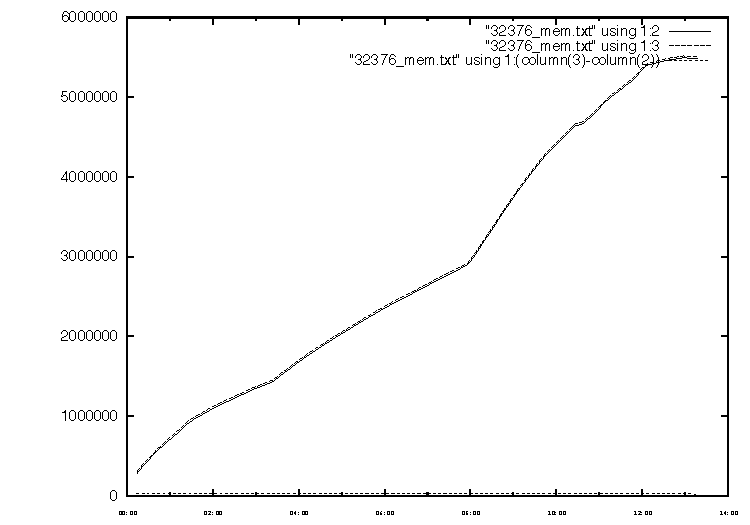
\includegraphics[width=\pdfwidth]{32376_mem.pdf}
 \caption{nyt.1000000.l3r0}
  \label{fig:32376_mem.pdf}
\end{figure}

The following plot (\figurename~\ref{fig:26251_mem.pdf}) shows the
memory use when using the above instance base for a classification
task. The test set consisted of \num{1000} lines of text from the same
Gigaword newspaper corpus.

\begin{figure}[!ht]
  \centering
  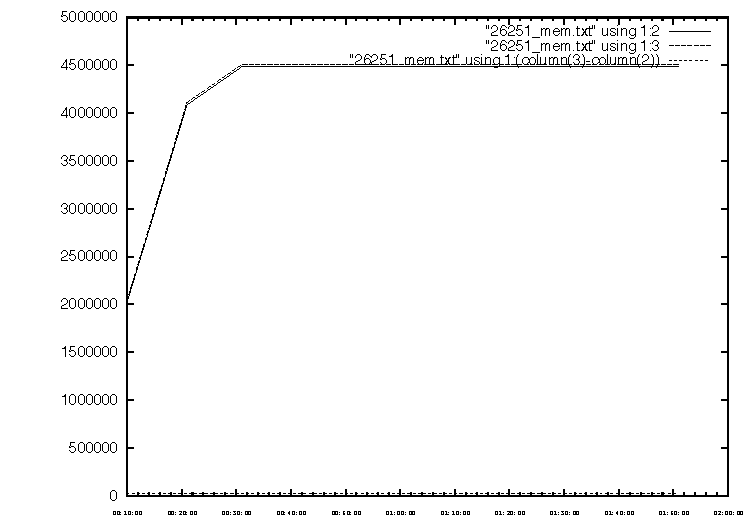
\includegraphics[width=\pdfwidth]{26251_mem.pdf}
 \caption{nyt.1000000.l3r0 ibase, test tail1000}
  \label{fig:26251_mem.pdf}
\end{figure}

\section{Comparison with \srilm{}}

The memory based approach to language modeling has several advantages
over a classical \ngram{}-based approach. First of all, we are not
limited to \ngram{}s but instead are able to use any number and type
of features in the instances. The instances can for example contain
grammatical and non-local context information. It is also possible to
use a right-context together, or even without, the words on the
left. 

Secondly, the tree-based approach has an inherent back-off
mechanism. In classical \ngram{}-models, a back-off to smaller
sequences (from trigrams to bigrams, to unigrams) is performed
when an \ngram{} is not found in the training data, typically when
unseen words are encountered. The \igtree{} algorithm returns the
distribution stored at that point in the tree when an unknown word is
encountered. The \triblt{} algorithm is more robust in that sense; it
continues to try to match the remaining feature values. 

In the following examples, we'll compare a \mb{} \lm{} with a \lm{}
generated by \srilm{}. 

\begin{comment}
We'll represent \wopr{} output like this;
an instance plus the target classification (in
grey), followed by the classification and distribution:\\ \\
  %\scalebox{0.95}{
\resizebox{!}{!}{ \wlr{w}{cg}{crazy
    when}{the}{}{the}{\dist{the}{526}\dist{he}{464}\dist{they}{219}\dsum{24}{2824}}}
\\The distribution is a list of tokens over their frequency. The top
figure after the $]$ shows the total number of elements in the
distribution. The bottom figure the sum of all the frequencies of the
distribution elements. In this example, \wopr{} predicted the correct
word \textsf{the} after \textsf{crazy when}. It returned a total of
\num{24} answers. The distribution can contain thousands of elements,
but we only show a handful of the top elements in our examples. If the
instance contains a right hand side context, it is shown after the
target. The next example shows \wopr{} output where the instance
contained right hand side context, and the wrong classification was
returned.\\ \\ \resizebox{!}{!}{\wlr{m}{ic}{crazy
    when}{the}{man}{a}{\dist{the}{488}\dist{a}{264}\dsum{8}{1244}}}\\An
incorrect classification is crossed out. A classification which is not
correct, but instead found in the distribution is marked with a dotted
line. 
%Finally, a \wex{} classification is marked with a small black
%dot in the upper left corner. Output from the \mono{} system is
%unmarked.
\end{comment}

\subsection{Logprob Comparisons}

% See README.compare_for_woprdoc

We created two \lm{}s, one with \wopr{} and one with \srilm{}. We used
\num{100000} lines of text from the Reuters corpus. For
\wopr{}, the context was set to \cmp{l2r0}. For \srilm{}, a third
order \lm{} was created. Test set was \num{1000} lines taken from
the same corpus.

%perl ../etc/pplx_px.pl -f rmt.5e5.t1000.l2r0_WOPRIGPPLX.px -l2 -r0 -L10

We take a sentence from the test data. First we show the \wopr{}
output. For each word in the test sentence we show the probability,
the $log_{2}$ and $log_{10}$ of the probability, followed by some
stats we will ignore for the moment.

%prob l10p md mal [bla] target
\begin{wout}{\wopr{} output}
0.07905  -3.6611  -1.1021  1 0 [00100] The
0.00324  -8.2712  -2.4899  1 0 [01000] only
0.05263  -4.2479  -1.2788  2 1 [01010] reason
0.37984  -1.3965  -0.4204  1 0 [00100] for
0.00008 -13.6354  -4.1047  1 0 [01000] caution
0.00451  -7.7941  -2.3462  2 1 [10010] is
0.01645  -5.9258  -1.7838  1 0 [01000] that
0.02150  -5.5394  -1.6675  1 0 [01000] we
0.01473  -6.0853  -1.8319  1 0 [01000] do
0.33673  -1.5703  -0.4727  1 0 [00100] not
0.03030  -5.0444  -1.5185  2 1 [01010] know
0.04545  -4.4594  -1.3424  2 1 [01010] what
0.00072 -10.4446  -3.1441  1 0 [10000] other
0.00004 -14.7434  -4.4382  1 0 [10000] demands
0.00002 -15.5113  -4.6694  1 0 [10000] Colston
0.00016 -12.6280  -3.8014  1 0 [10000] might
0.10623  -3.2348  -0.9738  1 0 [01000] have
0.00052 -10.8982  -3.2807  1 0 [01000] .
\end{wout}

And the \srilm{} output. The output is taken from the debug output from
\srilm{}. It shows the word (in context), followed by the size of the
matching \ngram{}, the probability and the $log_{10}$ of the probability.

\begin{wout}{\srilm{} output}
        p( The |  )               = [1gram] 0.00679429 [ -2.16786 ]
        p( only | The ...)        = [2gram] 0.00323679 [ -2.48989 ]
        p( reason | only ...)     = [3gram] 0.0205598 [ -1.68698 ]
        p( for | reason ...)      = [3gram] 0.384991 [ -0.41455 ]
        p( caution | for ...)     = [2gram] 2.32724e-05 [ -4.63316 ]
        p( is | caution ...)      = [1gram] 0.00198117 [ -2.70308 ]
        p( that | is ...)         = [2gram] 0.0164503 [ -1.78383 ]
        p( we | that ...)         = [3gram] 0.0625 [ -1.20412 ]
        p( do | we ...)           = [3gram] 0.00451603 [ -2.34524 ]
        p( not | do ...)          = [3gram] 0.65 [ -0.187087 ]
        p( know | not ...)        = [3gram] 0.024045 [ -1.61898 ]
        p( what | know ...)       = [2gram] 0.0868785 [ -1.06109 ]
        p( other | what ...)      = [1gram] 0.000100046 [ -3.9998 ]
        p( demands | other ...)   = [1gram] 1.4466e-05 [ -4.83965 ]
        p( Colston | demands ...) = [1gram] 5.8895e-06 [ -5.22992 ]
        p( might | Colston ...)   = [1gram] 6.02518e-05 [ -4.22003 ]
        p( have | might ...)      = [2gram] 0.106227 [ -0.973765 ]
        p( . | have ...)          = [2gram] 0.000162122 [ -3.79016 ]
\end{wout}

Normally, \srilm{} wraps each sentence in a \emph{start of sentence}
and \emph{end of sentence} marker. These have been switched off in
this comparison. The start-of-sentence marker is a bit like
our empty context markers which we insert before the first word(s) in
a sentence. 

\begin{wout}{$log_{10}$probablities compared}
-1.10209 -2.16786 1   11.6 [001] The
-2.48988 -2.48989 2    1.0 [000] only
-1.27875 -1.68698 3    2.6 [001] reason
-0.42039 -0.41455 3    1.0 [000] for
-4.10466 -4.63316 2    3.4 [001] caution
-2.34625 -2.70308 1    2.3 [001] is
-1.78383 -1.78383 2    1.0 [000] that
-1.66753 -1.20412 3    0.3 [010] we
-1.83187 -2.34524 3    3.3 [001] do
-0.47271 -0.18709 3    0.5 [000] not
-1.51851 -1.61898 3    1.3 [000] know
-1.34242 -1.06109 2    0.5 [000] what
-3.14414 -3.99980 1    7.2 [001] other
-4.43822 -4.83965 1    2.5 [001] demands
-4.66936 -5.22992 1    3.6 [001] Colston
-3.80140 -4.22003 1    2.6 [001] might
-0.97376 -0.97376 2    1.0 [000] have
-3.28069 -3.79016 2    3.2 [001] .
\end{wout}

Some predictions show a similar logprob from both \wopr{} and
\srilm{}. For examplme, both \lm{}s give the same likelyhood to the
second word in the sentence, \cmp{only}. Also the seventh word,
\cmp{that} gets similar logprobs. 

The difference is most likely due to \emph{smoothing} and
\emph{hapaxing}, which is done by \srilm{} but not by \wopr{}.

% See README.compare_for_woprdoc

\begin{comment}
In the next comparison, we show the results of a \triblt{} classifier on
the same data. 

%perl ../etc/pplx_px.pl -f rmt.5e5.t1000.l2r0_WOPRTRIBL2PPLX.px -l2 -r0 -L10 
\begin{wout}{\wopr{} \triblt{} output}
0.07907  -3.6608  -1.1020  1 1 [00110] The
0.00202  -8.9518  -2.6948  1 1 [01010] only
0.05263  -4.2479  -1.2788  1 1 [01010] reason
0.60000  -0.7370  -0.2218  1 1 [00110] for
0.00001 -16.3284  -4.9153  1 1 [10010] caution
0.00451  -7.7941  -2.3462  1 1 [10010] is
0.01645  -5.9258  -1.7838  1 1 [01010] that
0.06250  -4.0000  -1.2041  1 1 [01010] we
0.01156  -6.4346  -1.9370  1 1 [01010] do
0.65000  -0.6215  -0.1871  1 1 [00110] not
0.03030  -5.0444  -1.5185  1 1 [01010] know
0.04545  -4.4594  -1.3424  1 1 [01010] what
0.00072 -10.4446  -3.1441  1 1 [10010] other
0.00004 -14.7434  -4.4382  1 1 [10010] demands
0.00002 -15.5113  -4.6694  1 1 [10010] Colston
0.00016 -12.6280  -3.8014  1 1 [10010] might
0.10623  -3.2348  -0.9738  1 1 [01010] have
0.04196  -4.5747  -1.3771  1 1 [10010] .
\end{wout}

%perl ../etc/compare_px_srilm.pl -f rmt.5e5.t1000.l2r0_WOPRTRIBL2PPLX.px -s srilm.rmt.5e5.t1000.dbg2  -l2 -r0 -L10
\begin{wout}{\triblt{} versus \srilm{}}
-1.10201 -2.16786 1   11.6 [001] The
-2.69477 -2.48989 2    0.6 [000] only
-1.27875 -1.68698 3    2.6 [001] reason
-0.22185 -0.41455 3    1.6 [000] for
-4.91534 -4.63316 2    0.5 [000] caution
-2.34625 -2.70308 1    2.3 [001] is
-1.78383 -1.78383 2    1.0 [000] that
-1.20412 -1.20412 3    1.0 [000] we
-1.93702 -2.34524 3    2.6 [001] do
-0.18709 -0.18709 3    1.0 [000] not
-1.51851 -1.61898 3    1.3 [000] know
-1.34242 -1.06109 2    0.5 [000] what
-3.14414 -3.99980 1    7.2 [001] other
-4.43822 -4.83965 1    2.5 [001] demands
-4.66936 -5.22992 1    3.6 [001] Colston
-3.80140 -4.22003 1    2.6 [001] might
-0.97376 -0.97376 2    1.0 [000] have
-1.37713 -3.79016 2  258.8 [001] .
\end{wout}
\end{comment}

The trigrams generated by \srilm{} can also be read by \wopr{}, and
used instead of the \wopr{}-generated \ngram{}-model. The output can
then be compared with the \wopr{} \ngram{}-model. Doing this allows
\wopr{} to determine the distribution of the classifications, and
reciprocal ranking of the correct classification in the
distribution. The following table shows a comparison of \wopr{}
trigram-model scores and \srilm{} scores. The first two columns show
the \ltenp{} of the models. These are followed by the length of the
matching \ngram{}, and some statistics on the distributions, the last
two numbers are the \rr{}.

\begin{comment}
%from rmt.5e5.t1000_WOPR.ngd3
\begin{wout}{\wopr{} \ngram{} output}
The     -2.16785  1 77513 1728063 0.0625    [ ]
only    -2.48992  2  3096   11740 0.04      [ company 354 government 220 market 151 ]
reason  -1.27875  3    24      38 0.333333  [ thing 8 way 6 reason 2 ]
for     -0.221849 3     3       5 1         [ for 3 ( 1 I 1 ]
caution -4.10527  2  2630   12725 0.0172414 [ the 2774 a 931 their 169 ]
is      -2.34625  1 77513 1728063 0.0434783 [ ]
that    -1.7841   2   1466   7781 0.125     [ a 761 the 427 expected 391 ]
we      -1.20412  3    45     128 0.5       [ the 24 it 8 we 8 ]
do      -1.93702  3    37     173 0.1       [ have 37 will 24 are 21 ]
not     -0.187087 3     7      20 1         [ not 13 , 2 at 1 ]
know    -1.51851  3    69     165 0.333333  [ want 21 have 21 expect 15 ]
what    -1.34242  3    13      22 0.333333  [ if 3 the 3 a 2 ]
other   -3.14414  1 77513 1728063 0.00833333 [ ]
demands -4.43822  1 77513 1728063 0.00147929 [ ]
Colston -4.66936  1 77513 1728063 0.0014245  [ ]
might   -3.8014   1 77513 1728063 0.00213675 [ ]
have    -0.973765 2   101     273 0.5        [ be 67 have 29 not 29 ]
.       -3.28069  2   750    3817 0.0285714  [ been 653 to 297 a 271 ]
\end{wout}
\end{comment}

% Generated with: sh do_rmt.5e5.t1000_test.sh
%
% perl ../etc/compare_ngd.pl -w rmt.5e5.t1000_WOPR.ngd3 -s rmt.5e5.t1000_WOPRSRILM.ngd3 -L10
\begin{wout}{\ngram{}-models compared}
 -2.1679  -2.1679 1 1  77513  77513 1728063 1728063 0.062 0.062 The
 -2.4899  -2.4899 2 2   3096   3096   11740   11740 0.040 0.040 only
 -1.2788  -1.6870 3 3     24      4      38      18 0.333 0.333 reason
 -0.2218  -0.4145 3 3      3      1       5       3 1.000 1.000 for
 -4.1053  -4.3423 2 2   2630   2630   12725   12725 0.017 0.017 caution
 -2.3462  -2.3462 1 1  77513  77513 1728063 1728063 0.043 0.043 is
 -1.7841  -1.7838 2 2   1466   1466    7781    7781 0.125 0.125 that
 -1.2041  -1.2041 3 3     45     21     128     104 0.500 0.500 we
 -1.9370  -2.3452 3 3     37     20     173     156 0.100 0.100 do
 -0.1871  -0.1871 3 3      7      2      20      15 1.000 1.000 not
 -1.5185  -1.6190 3 3     69     25     165     121 0.333 0.333 know
 -1.3424  -1.0212 3 2     13     47      22     147 0.333 1.000 what
 -3.1441  -3.1441 1 1  77513  77513 1728063 1728063 0.008 0.008 other
 -4.4382  -4.4382 1 1  77513  77513 1728063 1728063 0.001 0.001 demands
 -4.6694  -4.6694 1 1  77513  77513 1728063 1728063 0.001 0.001 Colston
 -3.8014  -3.8014 1 1  77513  77513 1728063 1728063 0.002 0.002 might
 -0.9738  -0.9738 2 2    101    101     273     273 0.500 0.500 have
 -3.2807  -3.5967 2 2    750    750    3817    3817 0.029 0.029 .
\end{wout}

\begin{comment}
in wopr/doc:

SRILM:
/Users/pberck/work/srilm1.5.7/bin/macosx/ngram-count -no-eos -no-sos -text rmt.1e5 -sort -write rmt.1e5.nct -lm rmt.1e5.srilm
/Users/pberck/work/srilm1.5.7/bin/macosx/ngram -no-eos -no-sos -ppl rmt.t1000 -lm rmt.1e5.srilm -debug 2 > rmt.t1000.srilm_1e5_dbg2

WOPR TRIGRAM:
wopr -r ngl -p filename:rmt.1e5
wopr -r ngt -p ngl:rmt.1e5.ngl3f0,testfile:rmt.t1000,id:WOPR,topn:3,log:10

WOPRSRILM
wopr -l -r ngt -p ngl:rmt.1e5.srilm,ngc:rmt.1e5.nct,testfile:rmt.t1000,mode:srilm,id:WOPRSRILM,topn:3,log:10

WOPR IGTREE:
wopr -r make_ibase -p filename:rmt.1e5.l2r0,timbl:"-a1 +D"
wopr -r pplxs -p filename:rmt.t1000.l2r0,timbl:'-a1 +D',ibasefile:rmt.1e5.l2r0_-a1+D.ibase,id:WOPRIG

Resulting files:
  41968 -rw-r--r--    1 pberck  staff   21484750 30 aug 09:49 rmt.1e5.srilm
  49624 -rw-r--r--    1 pberck  staff   25403816 30 aug 09:49 rmt.1e5.nct
   2120 -rw-r--r--    1 pberck  staff    1081843 30 aug 09:51 rmt.t1000.srilm_1e5_dbg2
    792 -rw-r--r--    1 pberck  staff     403785 30 aug 09:55 rmt.t1000_WOPR.ngt3
    208 -rw-r--r--    1 pberck  staff     102656 30 aug 09:55 rmt.t1000_WOPR.ngp3
   1424 -rw-r--r--    1 pberck  staff     727788 30 aug 09:55 rmt.t1000_WOPR.ngd3
   1648 -rw-r--r--    1 pberck  staff     840877 30 aug 09:57 rmt.t1000.l2r0_5432.pxs
   2040 -rw-r--r--    1 pberck  staff    1043378 30 aug 09:57 rmt.t1000.l2r0_5432.px
   1648 -rw-r--r--    1 pberck  staff     840877 30 aug 09:59 rmt.t1000.l2r0_WOPRIG.pxs
   2040 -rw-r--r--    1 pberck  staff    1043378 30 aug 09:59 rmt.t1000.l2r0_WOPRIG.px
    848 -rw-r--r--    1 pberck  staff       423K 30 aug 10:52 rmt.t1000_WOPRSRILM.ngt3
    224 -rw-r--r--    1 pberck  staff       109K 30 aug 10:52 rmt.t1000_WOPRSRILM.ngp3
   1592 -rw-r--r--    1 pberck  staff       796K 30 aug 10:52 rmt.t1000_WOPRSRILM.ngd3

SCRIPTS:

WOPRIG vs SRILM: (compares the wopr igtree with srilm)
perl  ../etc/compare_px_srilm.pl -f rmt.t1000.l2r0_WOPRIG.px -s rmt.t1000.srilm_1e5_dbg2 -l2 -r0
...
000:  8326 ( 50.90%)
001:  3509 ( 21.45%)
010:  4523 ( 27.65%)
    ------
     16358

WOPR TRIGRAM vs WOPRSRILM (compares the plain wopr trigrams with srilm trigrams)
perl ../etc/compare_ngd.pl -w rmt.t1000_WOPR.ngd3 -s rmt.t1000_WOPRSRILM.ngd3 
...
Lines: 16358
Oov: 938
Equal logp: 9039
Equal n: 15566
Equal dcount: 13015
Equal sumf: 13011
Equal rr: 15740
Wopr:  0:938 1:5689 2:5690 3:4041 
Srilm: 0:938 1:5689 2:6482 3:3249 

WOPR TRIGRAM vs WOPRIG (compares plain wopr trigrams with wopr igtree)
perl ../etc/compare_ngd.pl -w rmt.t1000_WOPR.ngd3 -p rmt.t1000.l2r0_WOPRIG.px -l2 -r0
...
Lines: 16358
Oov: 938
Equal logp: 4491
Equal n: 5933
Equal dcount: 6263
Equal sumf: 6235
Equal rr: 8603
Wopr:     0:938 1:5689 2:5690 3:4041 
Srilm/PX: 0:866 1:9461 2:6031 

WOPRSRILM vs WOPRIG (compares srilm trigrams with wopr igtree)
perl ../etc/compare_ngd.pl -w rmt.t1000_WOPRSRILM.ngd3 -p rmt.t1000.l2r0_WOPRIG.px -l2 -r0 
...
Lines: 16358
Oov: 938
Equal logp: 3485
Equal n: 6445
Equal dcount: 4740
Equal sumf: 4724
Equal rr: 8282
Wopr:     0:938 1:5689 2:6482 3:3249 
Srilm/PX: 0:866 1:9461 2:6031 

--

do_rmt1_test.sh

"said": why is prob plain wopr trigrams different from igtree, which is
same as srilmtrigramsinwopr (and real srilm).

Dus: vergelijken IGTREE met NGT - zijn mss toch niet equivalent. Hm,
meer verschillen.

~/Downloads/a2pdf-1.13-OSX-Intel/a2pdf rmt.t1_WOPRSRILM.ngd3 >rmt.t1_WOPRSRILM.ngd3.pdf

line 4, small differences:
grep "and environmental" rmt.1e5.ngl3f0
Energy and environmental 3 0.333333

grep "and environmental" rmt.1e5.ngl3f0l10
Energy and environmental 3 -0.477121

grep "and environmental" rmt.1e5.srilm 
-3.424446	and environmental	-0.357372

MAAR in pxfile: -11.3758 (log2) naar p naar log10(p) geeft -3.4245,
en niet -3.42561 zoals in WOPR_ngd3

\end{comment}


\subsection{pplx}

The \igtree{} algorithm produces the following perplexity graph on the
English data (\figurename~\ref{fig:NY_pplx_-a1+D.pdf}).

\begin{figure*}[!ht]
  \centering
  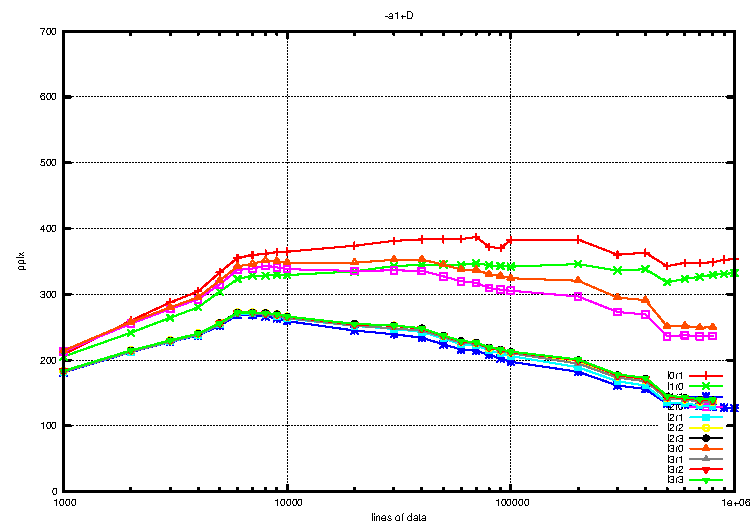
\includegraphics[width=\pdfwidth]{NY_pplx_-a1+D.pdf}
  \caption{Perplexity, \igtree{}}
  \label{fig:NY_pplx_-a1+D.pdf}
\end{figure*}

The perplexity score is low in the
beginning, due to the large number of unknown words. The only known
words are the function words, making up the skeleton of the
sentence. Most of the content words will still be unknown at this
point. As we train the classifier on more and more data, more of the
content words become known. This causes a rise in the perplexity score
first, before it starts to fall again.

The corresponding \srilm{} graph looks like this
(\figurename~\ref{fig:NY_pplx_slirm.pdf}). Note that \srilm{}
calculates two figures, one with (labeled pplx) and one without sentence
markers (labeled pplx1). 

\begin{figure*}[!ht]
  \centering         %gnuplot NY_pplx_srilm.plot
  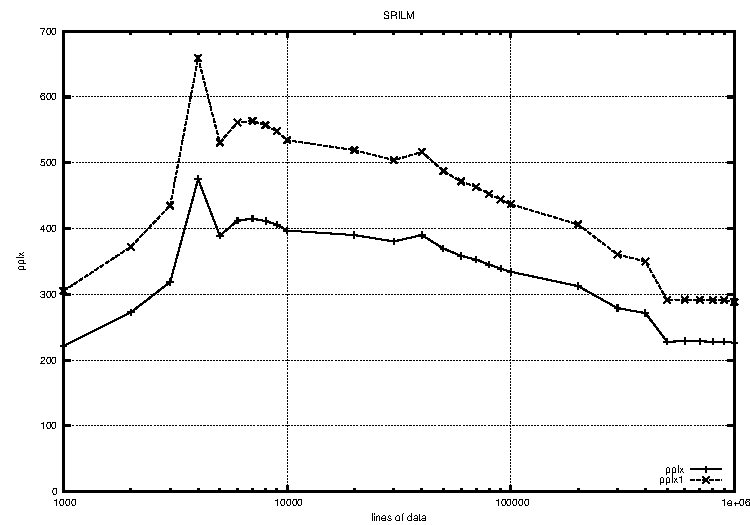
\includegraphics[width=\pdfwidth]{NY_pplx_slirm.pdf}
  \caption{Perplexity, \srilm{}}
  \label{fig:NY_pplx_slirm.pdf}
\end{figure*}

\chapter{Reference}

\section{Data}

\subsection{\cmp{window\_lr}}

Creates a \emph{windowed} data set. The \cmp{lc} and \cmp{rc}
parameters set the size (number of words) of the left and right
context. Out of sentence feature values will be filled with as many
\cmp{\_} (underscore character) as needed. \Wopr{} assumes the input
file contains one sentence per line. It will slide a window over each
sentence, and each word will be at the target position once. There is
an extra parameter \cmp{to}, which when set will let you predict the
next word after the next word. That is, if set to \num{1}, it will not
take the token at the window position as target, but the one to the
right. Setting it to \num{2} skips one more, \etc{}. The default value
for \cmp{to} is 0 so it can be left out if so desired.

\begin{varlist}{filename}
\item[filename] The file to window.
\item[lc] Left context. Number of words on the left side of the target.
\item[rc] Right context. Number of words on the right side of the target.
\item[to] target offset. Shift the target position to the right. Setting this to
  one will skip one word, that is, a b -> d, c will be skipped.
\end{varlist}

The output filename will have the context appended to it, in the form
\cmp{l3r0}. The \cmp{to} parameter will be appended if non-zero.

\subsection{\cmp{hapax}}

Hapaxing translates all tokes with a frequency less than or equal to
the \cmp{hpx} parameter to the string \cmp{$<$unk$>$}. For hapaxing we use
a previously created lexicon on a \emph{windowed} data set. The target
(i.e the last token on each line of data) is not hapaxed.

\begin{varlist}{filename}
\item[filename] The windowed data set to hapax.
\item[lexicon] The lexicon file to use.
\item[hpx] The frequency value.
\item[hpx\_sym] The symbol to use for hapaxed tokens. Defaults to
  \cmp{$<$unk$>$}. 
\end{varlist}

\subsection{\cmp{lexicon}}

Creates a lexicon file for the given text file. The lexcion consists
of a list of tokens, followed by its frequency.

\begin{varlist}{filename}
\item[filename] The data set to read.
\end{varlist}

It creates three output files, one with the suffix \cmp{.lex}
containing the lexicon, and one with \cmp{.cnt} containing counts of
counts. The first lines consists, for historical reasons, of three 
zeroes. The next line shows the number of tokens that occur once,
followed by the number of tokens that occur twice, \etc{}. Each line
contains the number of occurences, followed by the frequency, followed
by the number of occurences again. Only the first two columns are
interesting, the third was part of a now abandoned smoothing experiment.
The third file has the extension \cmp{.av} and contains a
anagram value for each word. The value is the sum over each letters'
\textsc{ascii} value to the power 5. This allows the rapid searching
of anagrams in a lexicon; the same letters will give the same value,
regardless of the order of the letters.

\begin{wout}{}
alerting 114508940294
altering 114508940294
integral 114508940294
relating 114508940294
triangle 114508940294
\end{wout}

\subsection{\cmp{rfl}}

This command outputs a range of words taken from a lexicon. The
entries in the lexicon are sorted by frequency. The highest frequency
comes first and has rank 1.  Because we take ranks, a range of ten
ranks can contain more than ten items as a number of words can have
the same rank.

\begin{varlist}{lexicon}
\item[lexicon] The lexicon file to process.
\item[n] Starting rank.
\item[m] Last rank.
\end{varlist}

\subsection{\cmp{lcontext}}

Create the global context part of the instances, and optionally merge
them with a normal data set.

\begin{varlist}{lexicon}
\item[filename] The normal data set or text file, depending on the
  value of the \cmp{gct} parameter.
\item[range] The file containing the words for the global context.
\item[gcs] Global context size
\item[gcd] Global context decay
\item[gco] Global context offset. Default to \cmp{0} which means that
  the global context starts directly after we have seen a word. This
  means that overlap between the normal and the global context is
  possible. The \cmp{gco} parameters introduces an extra offset of the
  specified number of instances. 
\item[gct] Global context type. Type \cmp{0}, the default, creates a
  global context consisting of words. Type \cmp{1} creates binary
  features. The latter means a binary value for every word in the
  \cmp{range} list supplied. The \cmp{gcs} parameter is ignored in
  this case. Type \cmp{2} creates a \q{hashed} value, that is, one
  value representing the words in the global context, in a position
  independent order.
\item[fd] Create from data (default \cmp{1}). Takes the words from a
  normal, windowed data set. Setting this to \cmp{0} creates global
  context from a normal text file.
\item[id] Identifier to append to the output filenames. If not
  specified, it defaults to the empty string.
\item[gc\_sep] Defaults to \cmp{1}, a space. This space is inserted
  between the binary (type \cmp{1}) feature values. Setting it to
  \cmp{0} concatenates all the binary features into one binary string
  feature. 
\end{varlist}

\subsection{\cmp{gap}}

A function to examine how words are distributed in a text. Can even be
used to generate data for the \emph{global context} data.

This function counts the number of tokens between the occurrences of
the words we are examining. A \cmp{gap} parameter is used to determine
whether words are \q{close} together or not. Two output files are
produced, one with suffix \cmp{gap} and one with suffix \cmp{gs}. The
gap size is appended to the suffixes. The first file contains a list
with words plus the gaps and a few statistics. Groups of small gaps
are enclosed between parenthesis, giving an idea of how the words are
clustered. The second file contains just the words and the statistics,
and can optionally be filtered on several parameters.

An example of the contents of the first file.

%pberck@scylla:/exp2/pberck/mrr$ /exp/pberck/wopr/wopr -r gaps -p filename:nyt.10000,lexicon:nyt.100000.lex,overwrite:1
\begin{wout}{\cmp{gap} output}
wines 13 ( 50 92 ) 395 ( 100 38 28 37 16 77 10 21 15 )
                            [ 2 3 0.666667 11 1 0.916667 484 44 8.97727 ]
\end{wout}

The example shows the token \cmp{wines}, which occurs \num{14} times
in the text. The first three (note that we show \emph{gaps}) are
\num{50} and \num{92} tokens apart (a \emph{close} group). Then there
is a large gap of \num{395} tokens until we come across the next
occurrence of \cmp{wines}. Then there is another group of \num{10}
occurrences close together.

The first two numbers in the statistics show the number of close
groups, and the number of potential groups. We have the two bracketed
groups represented by the first number. There could have been three
groups if the large gap in the middle had had an occurrence of
\cmp{wines} within the gap distance, so that makes the total
three. The number after that shows the ratio between those two
numbers. The next numbers, \num{11} and \num{1}, show we have \num{11}
close gaps and only one large gap. The ratio between the number of
close gaps and the total number of gaps is shown by the next
number. Note that with \num{13} occurrences of the token, we only have
\num{12} gaps. The number \num{484} is the sum of the close gaps
values, which in its turn is followed by the average close gap
distance. The last number is the ratio between the average large gap
size and the average small gap size.

The second file contains the same information as the first one, but
without the gaps.

\begin{wout}{\cmp{gs} output}
wines 13 2 3 0.666667 11 1 0.916667 484 44 8.97727
\end{wout}

This list can be filtered by setting the \cmp{filter} parameter to
\cmp{1}. Only tokens satisfying the conditions will be added to the
\cmp{gs} file. The \cmp{gap} file will still contain all the tokens
from the specified lexicon.

\begin{varlist}{lexicon}
\item[filename] A normal text file.
\item[lexicon] List of words to examine, in \wopr{}s lexicon format.
\item[gap] The maximum gap between tokens to consider them
  \q{together}.
\item[filter] A boolean to specify if we want to filer the \cmp{.gs}
  output. If set, the following conditions must be met for a word
  to be included in the output.
\item[min\_f] Minimum word frequency of words to include. Defaults to
  0. The token frequency must be larger or equal to this.
\item[max\_f] Maximum word frequency of words to include. Defaults to
  the maximum \emph{long} value the computer can handle. The token
  frequency must be less than this.
\item[min\_r] Minimum ratio between small and large gaps. Defaults to
  0.5. The ratio must be larger or equal to this.
\item[max\_r] Maximum ratio between small and large gaps. Defaults to
  1.1. It can never be more than 1, but the default will make sure it
  will be included. The ratio has to be less that this parameter.
\item[min\_a] Minimum average small gap value.
\item[max\_a] Maximum average small gap value.
\item[min\_p] Minimum groups to potential groups ratio.
\item[max\_p] Maximum groups to potential groups ratio.
\item[min\_g] Minimum average large to small groups size ratio.
\item[max\_g] Maximum average large to small groups size ratio. 
\end{varlist}

%woordn^5  =>?  woordx^5 + woordy^5 (collision)

\section{Training}

\subsection{\cmp{make\_ibase}s}

\begin{varlist}{filename}
\item[filename] Filename of the windowed data set.
\item[timbl] Settings for \Timbl{}. The parameters will be included in
  the name of the saved instance base file, with exception of the
  \cmp{k} parmeter which only affects processing a test set.
\end{varlist}

\subsection{\cmp{ngl}}

This creates a file with uni- to \ngram{}s for the given text
file. For each \ngram{}, the absolute frequency count and a
conditional probability is calculated. The \cmp{fco} parameter is a
frequency cut off value; only \ngram{}s which occur more often than
the specified \cmp{fco} parameter are included in the model.

\begin{varlist}{filename}
\item[filename] The text file to read.
\item[n] The largest \ngram{} to include. Default is \cmp{3}.
\item[fco] The frequency cut-off value, defaults to \cmp{0}.
\item[log] Output the $log_2$ or $log_{10}$ of the probability. Only
  two and ten are allowed.
\end{varlist}

The output file will have the extension \cmp{.ngl3f0}, both the
\cmp{n} and \cmp{fco} value are included. When specifying the
\cmp{log} parameter, the log value is appended too (\cmp{.ngl3f0l10}).

\section{Testing}

\subsection{\cmp{pplxs}}

The \cmp{pplxs} function is geared towards word prediction. It takes
an instance base, and calls \Timbl{} to process the test file. A
number of word prediction related values are calculated and written to
the output file.

It creates two output files, one with suffix \cmp{.px} and one with
suffix \cmp{.pxs}.  The \cmp{.px} output contains the following:

\begin{wout}{}
85 bp bp 0 0 1 cg k 1 1 1 11 1 [ bp 11 ]
bp over over 0 0 1 cg k 1 1 1 11 1 [ over 11 ]
over LIBOR Libor -16.4148 0 87364.5 ic k 1 1 1 11 0 [ Libor 11 ]
LIBOR delayed . -13.915 2.502 15452.2 ic k 1 1 8 44 0 [ . 14 , 11 for 6 ]
\end{wout}

The first tokens contain the instance (in this case \cmp{l1r0}),
followed by the classification. This is followed by the logprob of the
classification, the entropy of the distribution and the word level
perplexity (\wlp{}). The logprob is the $log_2$ of the probability of the
classification. The entropy of the distribution $D$ is calculated as
follows:

\begin{equation}
H(p) = -\sum_{x \in D} \, p(x)\log_2 p(x)
\label{eq:entropy}
\end{equation}

The word level perplexity is defined as:

\begin{equation}
\wlp{} = 2^{-p_{classification}}
\label{eq:wlp}
\end{equation}

These three numbers are followed by an indicator (\cmp{cg}, \cmp{cd}
or \cmp{ic}), followed by an known/unknown word indicator
(\cmp{k}/\cmp{u}). This is followed by the match-depth and a boolean
value indicating matched-at-leaf (one or zero). See
\cite{Daelemans+09} for a more thorough explanation. The following
three values are the distribution size, the sum of the distribution
frequencies, and the \emph{reciprocal rank} of the answer. Finally,
the output contains the top-$n$ of the distributions, specified as a
list of \cmp{token frequency} pairs.

The \cmp{.pxs} output contains a summary per line of input. It
contains the sentence number, followed by the number of words in the
sentence, the sum of the logprobs of the words, the average
perplexity, and the average \wlp{}. This is followed by
the number of unknown words in the sentence, the sum of the logprobs
of the known words and the standard deviation of the word level
perplexities. The final element in the output is a list with the
\wlp{} of each word in the sentence.

\begin{wout}{}
0 14 -113.718 278.73 30724.6 14 -113.718 75772.5 [ 594.087 105.375
                     181718 28.3925 392.646 116.143 1.61151 216331
                     2616.16 28.3925 28129.8 68.2397 2 11.6667 ]
\end{wout}

\begin{varlist}{ibasefile}
\item[filename] Test file to process.
\item[dir] Instead of one file, a whole directory with files will be
  processed if the \cmp{dir} parameter is specified instead of the
  \cmp{filename} parameter.
\item[dirmatch] A regular expression which determines which files will
  be read from the directory specified with \cmp{dir}.
\item[ibasefile] Filename of the instance base.
\item[timbl] Settings used to create the instance base.
\item[lexicon] Lexicon to determine known/unknown words.
\item[counts] Counts of ranks for the lexicon. This can be used to
  introduce smoothed or changed probabilities to the perplexity
  calculations. 
\item[hapax] Used when reading the lexicon.
\item[lc] Used to determine when a new sentence starts (for the
  \cmp{.pxs} output).
\item[rc] Used to determine when a new sentence starts (for the
  \cmp{.pxs} output). 
\item[topn] Number of elements from the \Timbl{} distribution to
  include in the output. Most frequent one first.
\item[cache] Number of elements in the cache (the default of three is
  good). 
\item[cth] Cache threshold: A distribution is not cached until it
  contains this many items.
\item[is] Include the whole sentence in the output (pxs).
\item[log] The base of the logarithm to do the calculations
  in. Defaults to two, can be set to ten with \cmp{log:10}.
\item[id] Identifier to append to the output filenames. If not
  specified, it defaults to the \pid{}.
\end{varlist}

\subsection{\cmp{gt}}

The \cmp{gt} function is a general test routine; it calls \Timbl{} and
writes the output to a file. The word prediction calculations are not
performed. The output filename is the name of the testfile, followed
by the \cmp{id} and the suffix \cmp{gt}.

The output contains the following:

\begin{wout}{}
million million cg 1 1 20 224 [ million 139 mln 30 billion 11 ]
\end{wout}

The first token is the target, the second the classification from
\Timbl{}. This is followed by an indicator (cg, cd, or ic), followed
by two values which indicate the match-depth, and a boolean value
specifying matched-at-leaf (one or zero). If the \cmp{topn} parameter
had been specified, this is followed by the distribution count, the
sum of the frequency of the elements in the distribution, and the
top-$n$ from the distribution. The latter is a list with
\cmp{token frequency} pairs.

\begin{varlist}{ibasefile}
\item[filename] Test file to process.
\item[dir] Instead of one file, a whole directory with files will be
  processed if the \cmp{dir} parameter is specified instead of the
  \cmp{filename} parameter.
\item[dirmatch] A regular expression which determines which files will
  be read from the directory specified with \cmp{dir}.
\item[ibasefile] Filename of the instance base.
\item[timbl] Settings used to create the instance base.
\item[cache] Number of elements in the cache (the default of three is
  good). 
\item[cth] Cache threshold: A distribution is not cached until it
  contains this many items.
\item[cs] Size of the cache which caches test instances. Default is
  \num{10000}. Note that this is a different cache from the cache which
  caches distributions. 
\item[topn] Number of elements from the \Timbl{} distribution to
  include in the output. Most frequent one first.
\item[id] Identifier to append to the output filenames. If not
  specified, it defaults to the \pid{}.
\end{varlist}

\subsection{\cmp{ngt}}

Apply an \ngram{} model to the test set. It finds the longest matching
\ngram{} from the supplied \ngram{}-model that fits.

\begin{varlist}{filename}
\item[filename] Filename of the plain text file to apply the model to.
\item[ngl] The \ngram{} model.
\item[ngc] File with counts from \srilm{}, see the \cmp{mode}
  parameter.
\item[mode] Switch to another mode, for example \cmp{mode:srilm} to
  use a language model generated by \srilm{}. When specifying an
  \srilm{} language model, a counts file needs to be specified with
  \cmp{ngc}. 
\item[n] Only \ngram{}s up to and including $n$ are used.
\item[id] Identifier to append to the output filenames. If not
  specified, it defaults to the empty string.
\item[topn] Number of elements from the distribution to
  include in the output. Most frequent one first.
\end{varlist}

It creates three output files, one with the extension \cmp{.ngp3}, one
with the extension \cmp{.ngp3}, and one with the extension
\cmp{.ngd3}. The \cmp{3} refers to the $n$-parameter supplied. The
\cmp{.ngt} output contains information per word in the text. The
\cmp{.ngp} file contains statistics per line of text, and the
\cmp{.ngd} file contains info about the distributions.

\subsection{\cmp{correct}}

Word correction based on contents of the distribution returned by the
classifier.

\begin{varlist}{max\_distr}
\item[filename] Test file to process.
\item[dir] Instead of one file, a whole directory with files will be
  processed if the \cmp{dir} parameter is specified instead of the
  \cmp{filename} parameter.
\item[dirmatch] A regular expression which determines which files will
  be read from the directory specified with \cmp{dir}.
\item[ibasefile] Filename of the instance base.
\item[timbl] Settings used to create the instance base.
\item[lexicon] Lexicon to determine known/unknown words.
\item[counts] Counts of ranks for the lexicon. This can be used to
  introduce smoothed or changed probabilities to the perplexity
  calculations. 
\item[mwl] Minimum word length (guess added if > mwl). Default 5.
\item[mld] Maximum levenshtein distance (guess added if <=
  mld). Default 1. Setting this to a larger value will introduce many
  potential misspellings.
\item[max\_ent] Max entropy of the distribution (guess added if <=
  max\_entropy). Default 5.
\item[max\_distr] Maximum size of the distribution (guess added if <=
  max\_distr). Default 10.
\item[min\_ratio] Ratio of the target lexical frequency versus the
  frequency of the words in the distribution. This is geared towards
  the disambiguation of confusibles and correctly spelt words on
  levenshtein distance one (like \cmp{woman} versus
  \cmp{women}). Default 0 (ignored).
\item[id] Identifier to append to the output filenames. If not
  specified, it defaults to the \pid{}.
\end{varlist}


\section{Miscellaneous}

\subsection{\cmp{generate}}

\begin{varlist}{ibasefile}
\item[start] Fill the starting context with this string. The default
  is to start generating from an empty context. It needs to contain as
  many words as specified in the \cmp{ws} parameter.
\item[filename] Output filename prefix.
\item[ibasefile] The instance base.
\item[timbl] The corresponding \Timbl{} settings.
\item[end] The end of sentence marker, defaults to a full stop.
\item[ws] The size of the left and right context added together.
\item[mode] A parameter to control if the next word taken from a
  number of possibilities is weighted according to frequency. Default
  is on (\cmp{1}). Setting it to \cmp{0} gives equal probability to
  each possibility.
\item[sc] Show the frequency count of each word.
\item[len] The maximum length of each sentence if the end of sentence
  marker is not reached.
\item[n] The number of sentences to generate.
\end{varlist}

\subsection{\cmp{server4}}

%../wopr -r server4 -p ibasefile:rmt.1e5.l2r0_-a1+D.ibase,timbl:"-a1 +D",lexicon:rmt.1e5.lex,mode:0
\begin{varlist}{cache\_size}
\item[ibasefile] The trained instance base.
\item[timbl] The corresponding \Timbl{} settings.
\item[lexicon] The corresponding lexicon.
\item[port] Port to listen on.
\item[mode] \cmp{mode:0}: input is an instance, \cmp{mode:1}: input is a
  sentence and will be windowed. In this case, see the \cmp{resm}
  parameter. 
\item[resm] \cmp{resm:0}: return average, \cmp{resm:1}: return sum, \cmp{resm:2}:
  return average, no OOV words.
\item[keep] \cmp{keep:1} does not close connection (for \pbmbmt{}).
\item[moses] \cmp{moses:1}: return a fixed width string for use in moses.
\item[lb] Log base of the answer, \cmp{lb:0}, returns a straight
  probability, \cmp{lb:10} returns the $log_{10}$.
\item[lc] Left context size for windowing.
\item[rc] Right context size for windowing.
\item[verbose] More output.
\item[hpx] Hapax level.
\item[skip\_sm] Remove sentence markers.
\item[cache\_size] Size of the cache. Received elements are cached,
  previous result is returned directly. Only useful when keep:1 is
  set. 
\end{varlist}

\bibliographystyle{apalike}
\bibliography{ilk}

\end{document}


